%==============================
\section{Online Adaptation}
\label{subsec:online-adaptation}

Since there are often uncertainties in the model, e.g., the agents may
transit faster or slower due to disturbances due to the additional constrains of self-loop $\sigma^s_\ell$,
an action might be finished earlier or latter,
or failures may occur during mission,
the optimal plan derived above might be invalid during online execution.
Thus, in this section, we first analyze these uncertainties in the execution time
and agent failures, for which online adaptation methods are proposed.

%==============================
\subsection{Online Synchronization under Uncertain Execution Time}\label{subsubsec:uncertain}
Uncertainty in the execution time can cause delay or early termination of subtasks.
Without proper synchronization, the consequences can be disastrous such as
one collaborative action is started without waiting for one
delayed collaborator.
To overcome these potential drawbacks, we propose an adaptation algorithm
that relies on \emph{online synchronization} and distributed communication.

More specifically, consider the optimal assignment~$J^\star$ and the local
sequence of subtasks for agent~$n$: $\tau_n=\omega^1_n\omega^2_n\cdots \omega^{K_n}_n$.
Without loss of generality, agent~$n$ just finished executing~$\omega^{k-1}_n$ and
is during the transition to perform subtask~$\omega^k_n$ at the designated region.
No matter how much the transition is delayed or accelerated,
the following synchronization procedure can be enforced to
ensure a correct execution of the derived plan even under uncertainties:

(i) \emph{Before} execution.
In order to start executing~$\omega^k_n$,
a ``\texttt{start}'' synchronization message is sent by agent~$n$ to agent~$m$,
for each subtask~$\omega^\ell_m$
satisfying~$(\omega^k_n,\,\omega^\ell_m)\in \preceq_{\varphi}$.
This message indicates that the execution of~$\omega^k_n$ is started
thus~$\omega^\ell_m$ can be started.
On the other hand, for each subtask~$\omega^\ell_m$
satisfying~$(\omega^\ell_m, \omega^k_n)\in \preceq_{\varphi}$,
agent~$n$ waits for the ``\texttt{start}'' synchronization message
from agent~$m$.
This message indicates that the execution of~$\omega^\ell_m$ is started
thus~$\omega^k_n$ can be started.
Last, for each subtask~$\omega^\ell_h$
satisfying~$\{\omega^k_n,\omega^\ell_h,\dots\}\subseteq \neq_{\varphi}$,
agent~$n$ checks the ''\texttt{start}'' or ``\texttt{stop}'' synchronization message
from agent~$h$ to ensure that not all subtasks in $\{\omega^k_n,\omega^\ell_h,\dots\}$ is executing.
Moreover, the self-loop constrain associated with the subsequent subtasks must be
followed to satisfy the poset.
Namely, each subset of agents that are executing~$\omega_{\ell'}$ publishes
the self-loop requirement~$\sigma^s_\ell$ associated with the subsequent subtask $\omega_\ell$.
It means that all other agents would satisfy the requirements in~$\sigma^s_\ell$
before~$\omega_{\ell'}$ is finished.


(ii) \emph{During} execution.
If~$\omega^k_n$ is a collaborative action, then
agent~$n$ sends another synchronization message to each collaborative agent
to start executing this action.
Otherwise, if~$\omega^k_n$ is a local action, then agent~$n$ starts the
execution directly;
(iii) \emph{After} execution.
After the execution of~$\omega^k_n$ is finished,
for each subtask~$\omega^\ell_h$
satisfying~$\{\omega^k_n,\,\omega^\ell_h,\dots\}\subseteq \neq_{\varphi}$,
a ``\texttt{stop}'' synchronization message is sent by agent~$n$ to agent~$h$,
This message indicates that the execution of~$\omega^k_n$ is finished
thus~$\omega^\ell_h$ can be started.
The above procedure is summarized in Fig.~\ref{fig:online adaption}.
The synchronization for collaborative tasks is easier as a collaborative
subtask can only start once all participants are present at the location.

%----------
\begin{remark}\label{remark:syn}
The synchronization protocol above is event-based,
i.e.,  only the subtasks within the partial relations
are required to synchronize,
which are much less than the complete set of subtasks.
\hfill  $\blacksquare$
\end{remark}
%----------


%==============================
\begin{figure}[t]
	\centering
	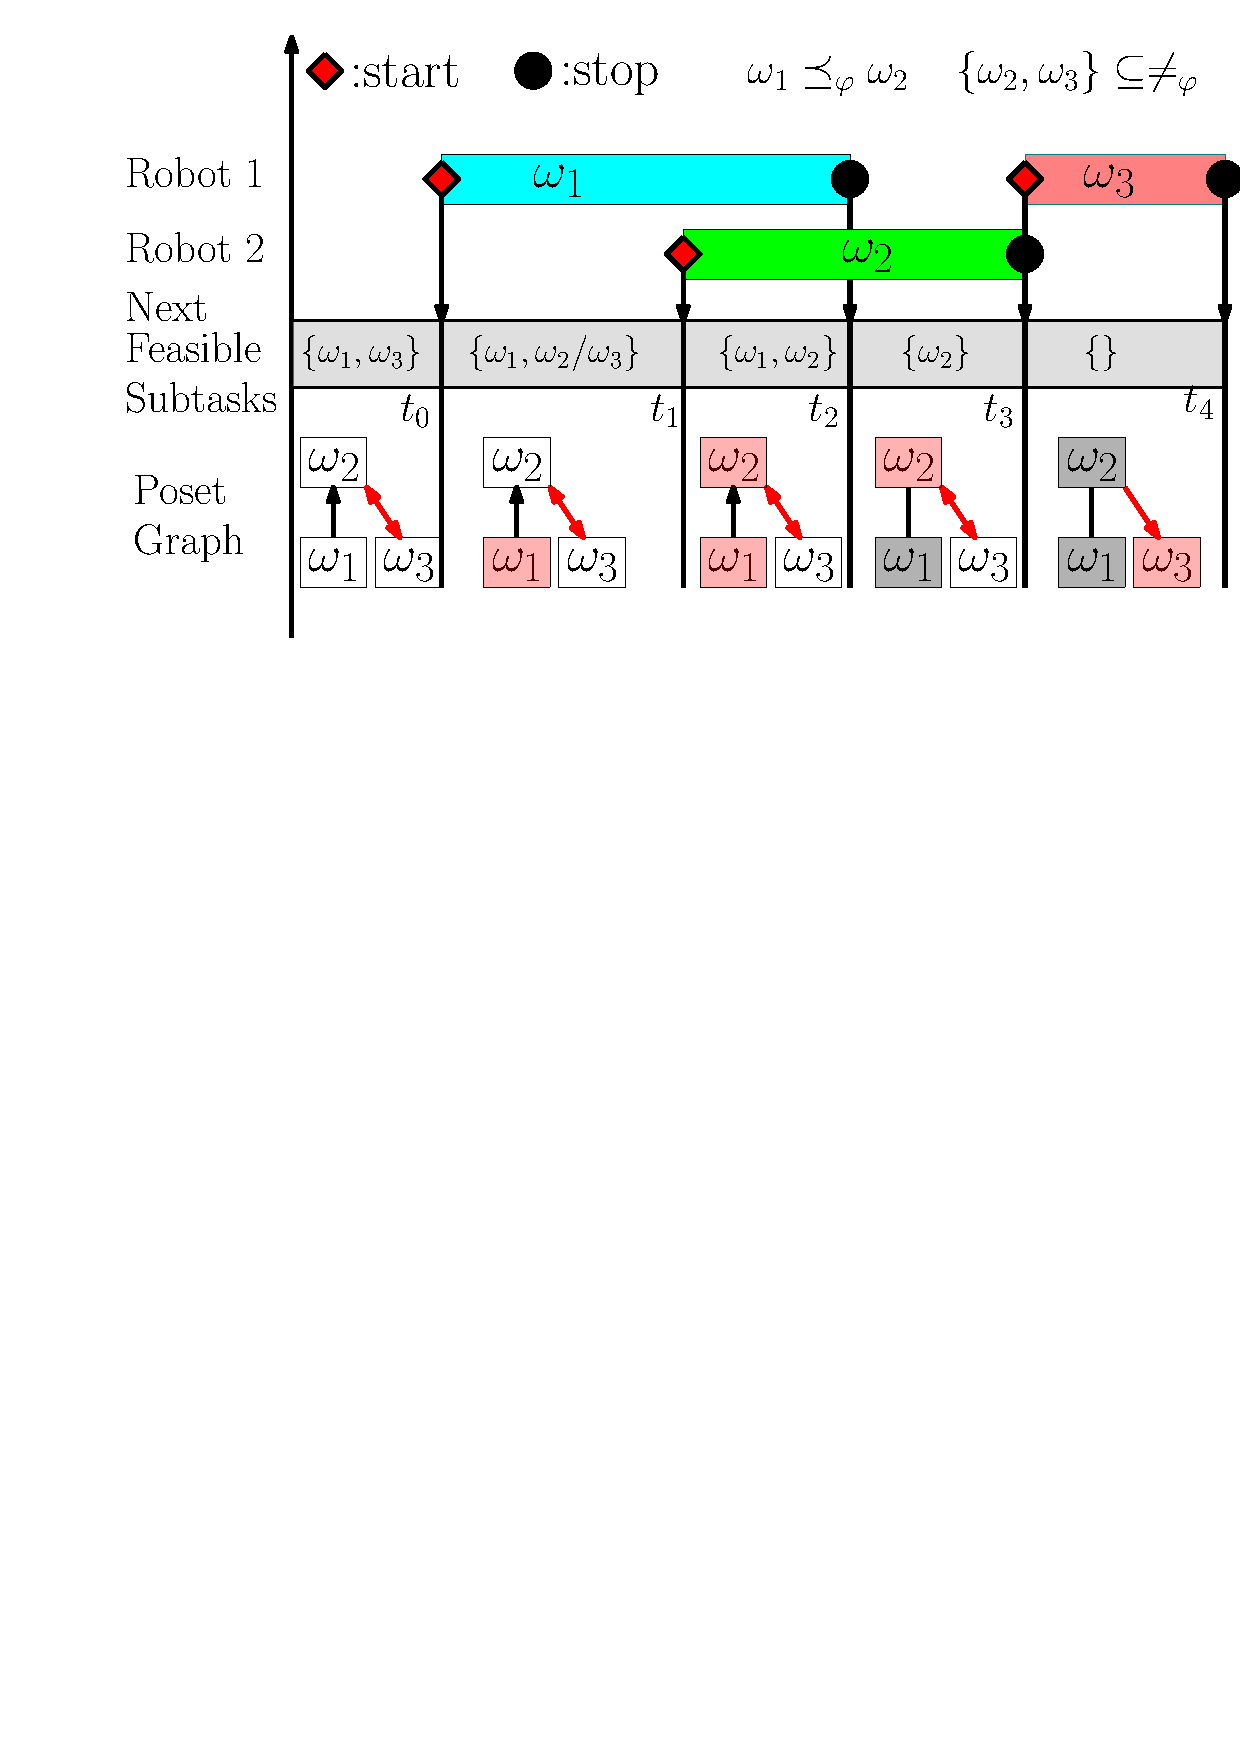
\includegraphics[width=0.7\linewidth]{figures/online_adapt3.pdf}
	%--------------------
        \caption{
Illustration of the online synchronization process
described in Sec.~\ref{subsubsec:uncertain}.
Consider the constraints~$\omega_1 \preceq_{\varphi}\omega_2$
and~$\{\omega_1, \omega_3\}\subseteq\neq_\varphi $.
The ``\texttt{Start}'' and ``\texttt{Stop}'' messages are
marked by red diamonds and black circles, respectively. The agent can only
execute the subtask if all relevant partial relation is satisfied.}
\label{fig:online adaption}
	%--------------------
\end{figure}
%==============================


%==============================
\subsection{Plan Adaptation under Agent Failures}\label{subsubsec:failure}
Whenever an agent is experiencing motor failures that it can not
continue executing its remaining subtasks,
a more complex adaptation method is required as the unfinished subtasks
should be re-assigned to other agents.

Assume that agent~$N_d$ has the optimal
plan~$\tau_{N_d}=\omega^1_{N_d}\omega^2_{N_d}\\\cdots \omega^{K_{N_d}}_{N_d}$.
It fails at time $t=T_d$ after the execution of subtask~$\omega^{k_d-1}_{N_d}$ and during the
transition to subtask~$\omega^{k_d}_{N_d}$.
Consequently, the set of unfinished tasks is given by:
\begin{equation}\label{eq:unfinished}
\widehat{\Omega}_{N_d}=\{\omega^{k'}_{N_d},\,k'=k_d,k_d+1,\cdots,K_{N_d}\},
\end{equation}
which is communicated to other agents before agent~$N_d$ failed.
Note that if an agent fails during the execution of a subtask,
this subtask has to be re-scheduled and thus re-executed.



Given this set of subtasks, the easiest recovery is to recruit another new
agent~$N'_d$ with the same capabilities as agent~$N_d$ and
takes over all tasks in~$\widehat{\Omega}_{N_d}$.
However, this is not always feasible, meaning that~$\widehat{\Omega}_{N_d}$ needs to
be assigned to other existing agents within the team.
Then, the BnB algorithm in Alg.~\ref{alg:BnB} is modified as follows.
First, the initial root node now consists of the subtasks that are already
accomplished by each functional agent, i.e.,
\begin{equation}\label{eq:new-initial}
  \nu'_0=(\tau'_1,\cdots,\tau'_{N_d-1},\tau'_{N_d+1},\cdots,\tau'_{N}),
\end{equation}
where~$\tau'_n=\omega^1_n \omega^2_n\cdots \omega^{K_n}_n$ and $K_n$ is last
subtask be accomplished at time $t=T_d$,
for each agent~$n=1,\cdots,N_d-1,N_d+1,\cdots,N$.
Namely, agent~$N_d$ is excluded from the node definition.
Second, the node expansion now re-assigns all unfinished tasks:
$
  \widehat{\Omega}_d= \bigcup_{n\in \mathcal{N}}\,\widehat{\Omega}_n,
$
where~$\widehat{\Omega}_n\subset \Omega_{\varphi}$ is the set of unfinished tasks
for agent~$n\in \mathcal{N}$, defined similarly as in~\eqref{eq:unfinished}.
Namely, each remaining task is selected according to the \emph{same} partial
ordering constraints~$P_{\varphi}$ as before agent failure, for node expansion.
Afterwards, the same branching rules and more importantly,
the methods for calculating lower and upper bounds are followed.
Consequently, an adapted plan~$\widehat{J}^\star$ can be obtained
from the same anytime BnB algorithm.
It is worth noting that the above adaptation algorithm shares the same
completeness and optimality property as Alg.~\ref{alg:complete}.

